 %% main.tex --- "Transferring and Reading Skills in Language Model Contexts"
%% Submission format: The ACM Web Conference 2027 (WWW '27), research track.
%%
%% The track asks for \documentclass[sigconf, anonymous, review]{acmart}
%% and caps a long paper at 8 pages of main content plus references and an
%% optional appendix, 12 pages in total, with the first 8 pages self-contained.
%% See https://www2027.thewebconf.org/research-track-papers/
%%
%% Layout of this project
%%   main.tex              this file: preamble, metadata, document skeleton
%%   sections/             main text, one file per section
%%   appendix/             appendices, one file per theme
%%   tables/               tabulars written by the generators in tools/
%%   figures/              figures written by the generators in tools/
%%   skillvector.bib       bibliography
%%
%% Build:  latexmk -pdf main.tex      (or ./build.sh from the repository)

\PassOptionsToPackage{table}{xcolor}
\documentclass[sigconf, anonymous, review]{acmart}

%% ------------------------------------------------------------------ rights
%% Anonymous review metadata; assigned publication identifiers are omitted.
\setcopyright{none}
\copyrightyear{2027}
\acmYear{2027}
\acmDOI{}
\acmConference[WWW '27]{Proceedings of the ACM Web Conference 2027}%
  {May 10 to 14, 2027}{Dublin, Ireland}
\acmISBN{}
\settopmatter{printacmref=false}

%% -------------------------------------------------------------- packages
%% acmart already loads graphicx, booktabs, xcolor, hyperref, url and natbib.
\usepackage{amsmath}
% libertine (loaded by acmart) already defines \Bbbk, and amssymb redefines it.
\let\Bbbk\relax
\usepackage{amssymb}
\usepackage{multirow}
\usepackage{tabularx}
\usepackage{placeins} % Keep each experimental stage with its displays.
\usepackage{tikz}
\usetikzlibrary{arrows.meta,positioning,calc}
% Shared table system: unshaded rows, generous spacing, restrained rules.
\definecolor{TableInk}{HTML}{284A63}
\definecolor{TableHeader}{HTML}{EAF0F6}
\definecolor{TransferHighlight}{HTML}{E4F1ED}
\definecolor{ConflictHighlight}{HTML}{FFF0DD}
\definecolor{TableStripe}{HTML}{F5F8FA}
\usepackage{etoolbox}
% Use periods between displayed CCS concepts, matching the manuscript prose.
\makeatletter
\patchcmd{\ccsdesc@parse}{\else; \fi}{\else. \fi}{}{}
\makeatother
\AtBeginEnvironment{tabular}{%
  \normalfont\rmfamily\fontsize{9}{11}\selectfont%
  \renewcommand{\arraystretch}{1.22}%
  \setlength{\aboverulesep}{2pt}%
  \setlength{\belowrulesep}{2.5pt}%
  \setlength{\heavyrulewidth}{0.7pt}%
  \setlength{\lightrulewidth}{0.3pt}%
  \arrayrulecolor{TableInk}%
}
\graphicspath{{figures/}}

%% Allow the four main figures and compact appendix table to float cleanly.
\renewcommand{\topfraction}{0.9}
\renewcommand{\bottomfraction}{0.9}
\renewcommand{\textfraction}{0.06}
\renewcommand{\floatpagefraction}{0.75}
\renewcommand{\dbltopfraction}{0.9}
\renewcommand{\dblfloatpagefraction}{0.7}
\setcounter{topnumber}{4}
\setcounter{bottomnumber}{3}
\setcounter{totalnumber}{6}
\setcounter{dbltopnumber}{4}

%% ---------------------------------------------------------------- macros
% A visible marker for numbers that are not in yet. Must be empty at submission.
\newcommand{\PEND}[1]{\textcolor{red}{[pending: #1]}}
\newcommand{\dvec}{\ensuremath{d}}
\newcommand{\gvec}{\ensuremath{g}}
\newcommand{\tvec}{\ensuremath{t}}

%% Long inline lists such as $0.06, 0.00, 0.62, 0.94$ carry no legal break point,
%% and in a 241pt column they run into the gutter. Make the comma a mild break
%% opportunity in maths only; TeX still prefers an ordinary interword break.
\mathchardef\mathcommachar\mathcode`\,
\mathcode`\,="8000
{\catcode`\,=\active \gdef,{\mathcommachar\discretionary{}{}{}}}
\emergencystretch=1em
% Avoid one- and two-letter fragments in the narrow review columns.
\AtBeginDocument{\lefthyphenmin=3\righthyphenmin=3}
\hyphenation{skill skills identify different}

%% Submission only. Historical extended sources remain archived in the repo.
%% References to those historical diagnostics use their descriptive fallback.
\newcommand{\extref}[3]{#3}

\begin{document}

\title{Still Needed, Hard to Transfer: Using and Reusing Contextual Skills}

\author{Anonymous Author(s)}
\affiliation{%
  \institution{Anonymous Institution}
  \country{}
}
\email{anonymous@example.com}

\begin{abstract}
Language models can adapt to new tasks by following instructions provided in context.
Reusing the internal states formed from these instructions could allow the resulting task capabilities to be shared across executions.
However, it remains unclear how the ability to transfer these states relates to the model’s continued dependence on the instructions.
We study this relationship using skills, sets of instructions that describe how to perform a task.
At different layers, we transfer states at the instruction positions from an execution using the correct skill into one using an unrelated skill.
Separately, we block attention to the skill in the original execution.
Across four models and two benchmarks, all eight comparisons show that transfer weakens at later layers while the original execution remains strongly dependent on the skill.
We then augment state transfer with key/value caches, the stored information used by attention.
At layer 16, this joint intervention improves accuracy over state transfer alone by 6.8 to 43.4 percentage points across all eight combinations.
For Qwen3-8B/MedCalc, accuracy rises from 3.5\% to 42.1\%, and blocking subsequent skill reading reduces it to 7.0\%.
These findings establish a separation between using contextual skills and reusing their internal states, and demonstrate cache-assisted recovery across models and tasks.
\end{abstract}


%% TODO before submission: regenerate from the ACM CCS tool at
%% https://dl.acm.org/ccs and paste the block it produces.
\begin{CCSXML}
<ccs2012>
   <concept>
       <concept_id>10010147.10010178.10010179</concept_id>
       <concept_desc>Computing methodologies~Natural language processing</concept_desc>
       <concept_significance>500</concept_significance>
       </concept>
   <concept>
       <concept_id>10010147.10010178.10010187</concept_id>
       <concept_desc>Computing methodologies~Knowledge representation and reasoning</concept_desc>
       <concept_significance>300</concept_significance>
       </concept>
</ccs2012>
\end{CCSXML}
\ccsdesc[500]{Computing methodologies~Natural language processing}
\ccsdesc[300]{Computing methodologies~Knowledge representation and reasoning}

\keywords{agent skills, Web agents, large language models, in-context learning,
activation patching, context reuse, mechanistic interpretability}

\maketitle

%% ================================================================ main text
% Insert early so the single-column float can occupy the first page's
% right-column top, alongside the abstract, using standard ACM float placement.
\begin{figure}[t]
\centering
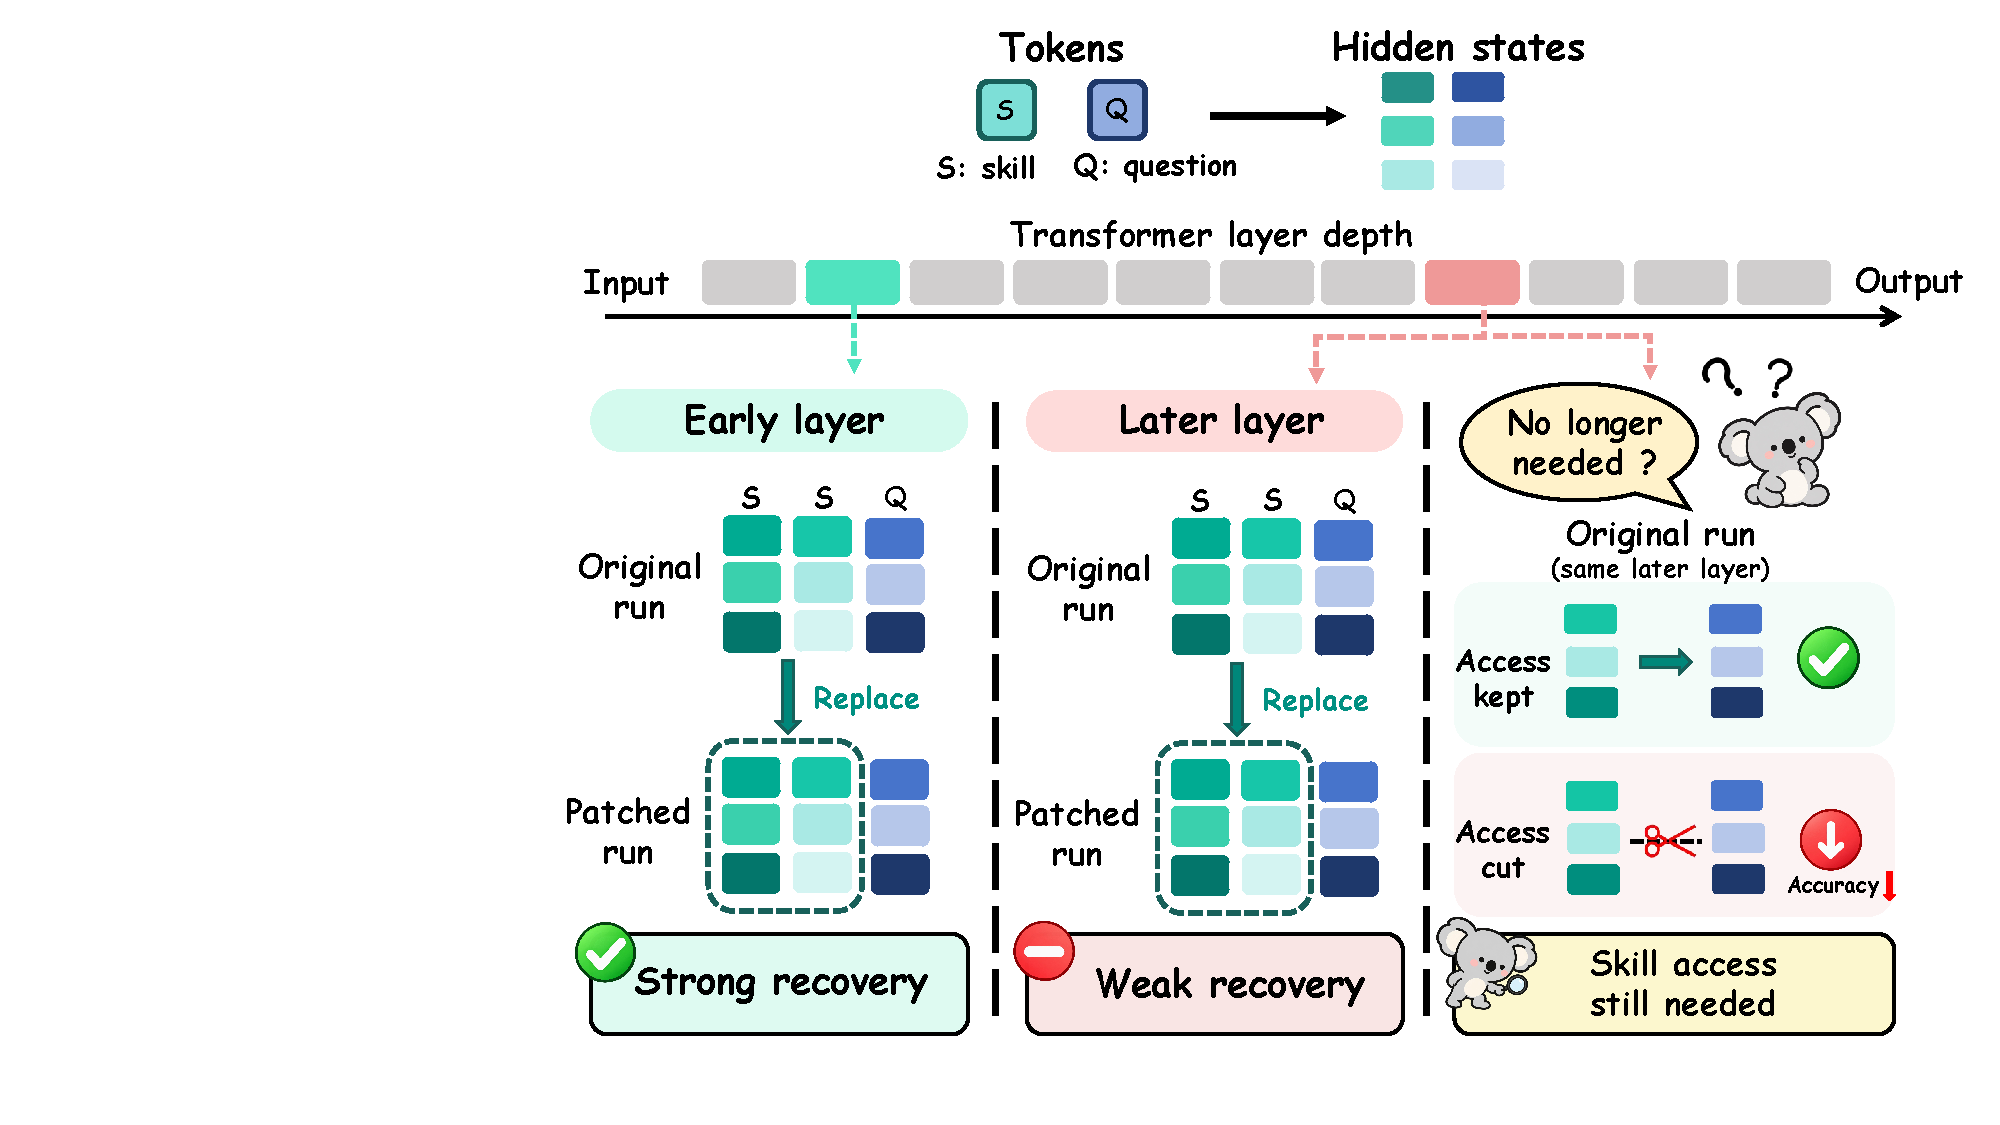
\includegraphics[width=\columnwidth]{fig-teaser.pdf}
\caption{Weak transfer and continued skill use at the same later depth.
Copying skill-position states from a correct-skill run into an unrelated-skill
run gives strong early recovery (left) and weak late recovery (middle).
At that same later depth, the original run still needs skill access:
retaining access preserves performance, while cutting it reduces accuracy
(right). S and Q label skill and question tokens.
Figure~\ref{fig:transferreading} gives the measured depth profiles.}
\Description{A schematic follows transformer depth from input to output.
At an early layer, replacing skill-position hidden states yields strong
recovery. At a later layer the same type of replacement yields weak recovery.
In the original correct-skill run at that later layer, retaining skill access
preserves performance while cutting access reduces accuracy. Green blocks
represent skill tokens and blue blocks question tokens.}
\label{fig:teaser}
\end{figure}

\section{Introduction}
\label{sec:intro}

Language models can perform new tasks by following instructions in their
context. A skill makes such instructions reusable: a calculator skill,
for example, specifies a formula, input conventions and the steps for
applying them to a new question. A model divides text into tokens and
represents each position with an internal vector, or hidden state.
If the hidden states formed from these
instructions also support reuse, one execution could supply task-relevant
information to another without changing the model's weights.

Agent Skills organize instructions, scripts and resources around a
\texttt{SKILL.md} entry point \citep{zhang2025agentskills}.
Web agents use reusable skills and workflows to guide later actions
\citep{wang2024awm,wang2026webxskill}. This motivates studying whether the
internal states formed from such instructions can also be reused. We
study this question through controlled question answering after a skill
has been selected, isolating the use and transfer of its instructions.

The difficulty is interpreting a failed transfer. If copying a skill's
hidden states no longer restores performance, has the model stopped
needing those instructions, or has the copy failed to supply what the
receiving execution needs? Task vectors summarize task demonstrations,
while function vectors combine selected internal attention outputs.
Both show that internal states can transmit task behaviour across contexts
\citep{hendel2023taskvectors,todd2024functionvectors}. Yet restoring an
execution and disrupting a successful one measure different effects
\citep{heimersheim2024patching}. This motivates our central question:
\emph{can skill-state transfer weaken while the original execution still
relies on access to the skill?}

We answer this question with two tests across model depth. The first
copies hidden states at the skill's token positions from a correct-skill
execution into an execution using length-matched text from an unrelated skill. The
second blocks attention to the skill in the original correct-skill
execution, from a chosen layer onward. Content, position and cross-question
controls first establish that early copying transfers skill-relevant
information. We then find a consistent separation in eight evaluated
combinations of four models and two benchmarks: transfer weakens at later
layers while the original execution remains strongly dependent on skill
attention (Figure~\ref{fig:teaser}).

We next test whether adding information omitted by hidden-state copying
can improve late transfer. Attention stores information from previously
processed tokens in a key/value (KV) cache. At layer $16$, copying these
caches together with hidden states improves accuracy over state transfer
alone in all eight settings, by $6.8$ to $43.4$ percentage points.
Blocking subsequent skill reading reduces the recovered accuracy in each
setting. For Qwen3-8B/MedCalc, joint replacement raises accuracy from
$3.5\%$ to $42.1\%$, and the reading cut reduces it to $7.0\%$.
The shared direction across models and tasks establishes cache-assisted
partial restoration alongside continued use of the skill.

The paper follows three steps: validate early transfer
(\S\ref{sec:battery}), establish its separation from continued skill use
(\S\ref{sec:depth}), and test the extent of cache-assisted restoration
(\S\ref{sec:mechanism}). Together, the tests distinguish the ability to
use contextual instructions from the ability to reuse their internal
states, and identify cached information as a component that improves reuse.

\section{Related Work}
\label{sec:related}

\paragraph{State transfer and its interpretation.}
Task vectors summarize demonstrations as internal vectors
\citep{hendel2023taskvectors}, and function vectors identify attention
outputs that transmit task behaviour \citep{todd2024functionvectors}.
Instructions also yield transferable components
\citep{davidson2025prompting,bigoulaeva2026instructionvectors}, whose effects
vary with intervention depth \citep{jit2025taskrepr}. Activation patching,
which copies internal states between executions, requires matched controls
and careful implementation
\citep{zhang2023bestpractices,heimersheim2024patching}. In particular,
restoring behaviour and disrupting it need not reveal the same components.
Interactions with other components can also affect a patching estimate
\citep{vaidyanathan2026mediators}. We use these methodological distinctions to compare skill-state transfer
and source dependence across depth.

\paragraph{Depth, source access and context caches.}
Pola and Balasubramanian \citep{onset2025instruction} locate an onset beyond
which selected hidden-state replacements largely cease to change answers in their
instruction tasks. Sia et al.\ \citep{sia2024incontexttranslation} use
layer-wise context masking, which blocks attention to selected context
positions, in machine translation and code generation to
locate where attention to the instructional context becomes unnecessary.
Joint transfer and masking analyses also locate subtask computation
\citep{yang2025internalcot}. We instead define the source as an explicit
skill-instruction span and compare transfer into a wrong-skill execution
with blocking attention to that span in the original execution on common questions.
The comparison measures how the two effects separate across depth.

PrefillNotes \citep{li2026prefillnotes} studies editable and reusable KV
caches. In its field-editing tasks, replacing local KV entries can fail
when downstream cached conclusions still reflect the old field. It also
composes precompiled skill caches into new contexts. Our focus is the
depth separation between skill-state transfer and original-run source
dependence. We then ask whether copying source caches together with
states partially restores late transfer.

\paragraph{Skills and reusable context.}
Agent Skills organize instructions and resources for on-demand use
\citep{zhang2025agentskills}. Benchmarks study skill retrieval and application
\citep{su2026srabench,skillsbench2026,sweskills2026}, while matched-budget
evaluations expose their dependence on available computation
\citep{hajimiri2026budgetskills}. We hold skill selection fixed.
Other approaches compress context into aggregated activations
\citep{ardoin2026promptcompression}, learned summary tokens
\citep{mu2023gist}, hidden states \citep{ge2024icae}, or weight updates
\citep{doc2lora2026,deepcontextdistill2025}. Our interventions characterize
naturally occurring states and source dependence without training a
compression mechanism.

\section{Problem Formulation}
\label{sec:formulation}

\paragraph{Skills, executions and token positions.}
We supply a skill's instructions directly and hold skill selection fixed.
For the same question, the \emph{donor} execution uses the correct skill
and the \emph{receiver} execution uses length-matched text from a fixed
unrelated skill (Appendix~\ref{app:detail}). The skill's token positions, denoted $\mathcal I$, form the
\emph{source span}. For example, a calculator's formula and input
conventions belong to this span. The question does not.
\emph{Readers}, denoted $\mathcal J$, are positions after the source span, including subsequent
prompt tokens and generated answer tokens. Thus receiver names an
execution, whereas reader names a token position that can attend to the
skill. Causal attention prevents a position from reading future tokens,
so tokens before the source cannot read it.

Layers are indexed from zero. The model processes prompt tokens during
\emph{prefill} and generates answer tokens during \emph{decoding}.
We use greedy decoding, which selects the highest-probability next token.
Our main comparison asks what transferring source states restores in the
receiver and what blocking source attention removes from the donor.

% Queue the design graphic within the methods, ahead of the next page top.
\begin{figure*}[t]
\centering
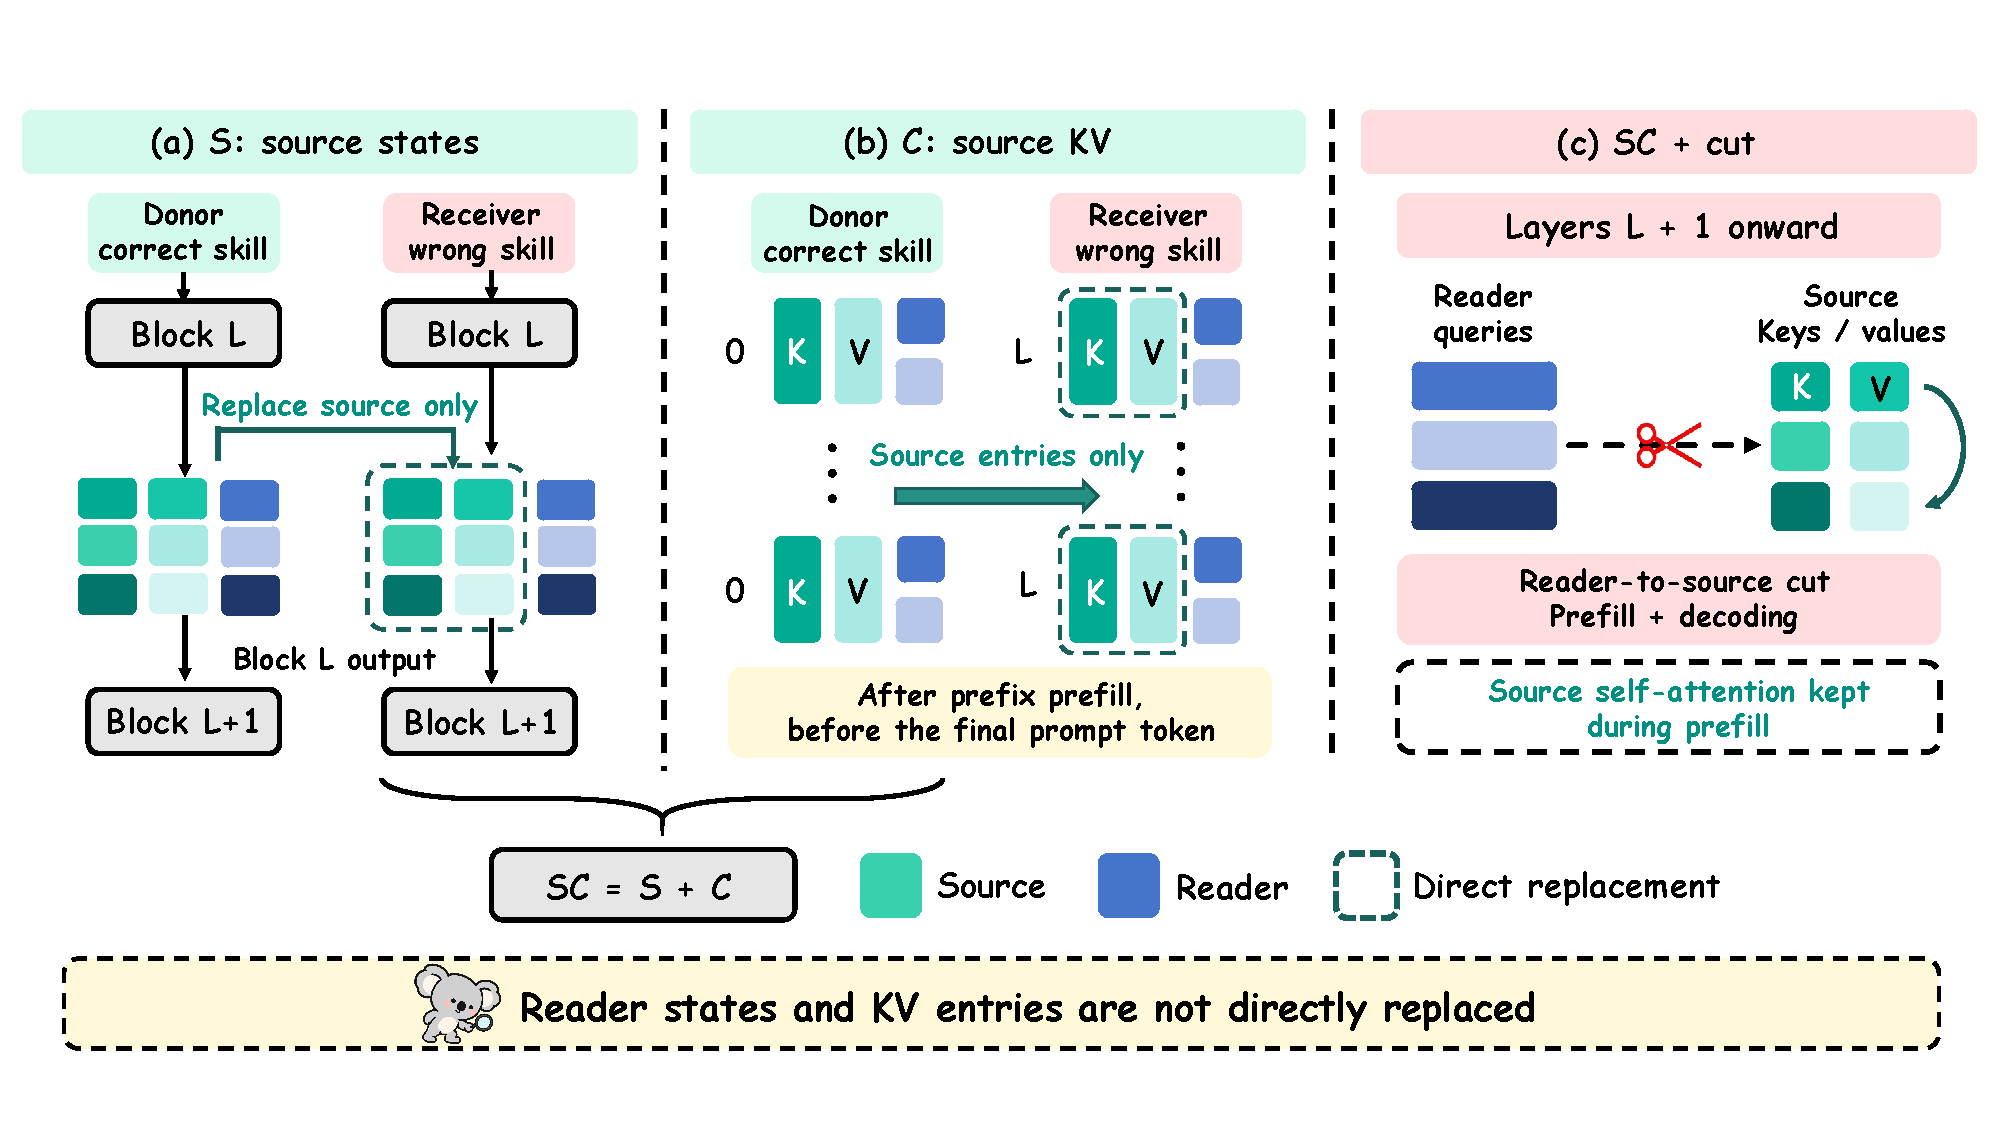
\includegraphics[width=\textwidth]{fig-intervention-design.pdf}
\caption{Timing of state repair, cache repair and the reading cut in the receiver.
The prefix contains all prompt tokens except the last.
(a) $S$ copies donor source states at block $L$'s output during prefix prefill.
(b) $C$ copies source-position key/value (KV) entries at layers $0$ through
$L$ after prefix prefill, before final-token recomputation. $SC$ combines
these two writes, then recomputes the final prompt token and generates.
(c) $SC+\mathrm{cut}$ installs a reading mask before prefill, blocking
reader-to-source attention from $L+1$ onward during prefill and decoding.
Source-to-source attention remains unmasked. Reader states and caches
evolve through computation rather than direct replacement.
Figure~\ref{fig:mechanism}(b) separately tests cuts in the original correct-skill run.}
\Description{Three panels illustrate source-state replacement at block L's
output, source-key/value replacement at layers zero through L, and joint
replacement with a reader-to-source attention cut from layer L plus one.
Green cells mark source positions, blue cells mark readers, and dashed teal
outlines mark direct replacements. The cut applies during prefill and
decoding while source self-attention remains unmasked during prefill.}
\label{fig:design}
\end{figure*}

\paragraph{Hidden-state transfer.}
Each Transformer block is a processing layer that updates the token
vectors. Let $H^L$ denote its output at layer $L$, also called residual
states. Subscripts $D$ and $R$ denote donor and receiver.
State replacement, labelled $S$, writes
\begin{equation}
S:\qquad H_R^L[\mathcal I]\leftarrow H_D^L[\mathcal I].
\label{eq:inject}
\end{equation}
The write occurs during prefill, after which the receiver continues with
the patched states. Other positions at that layer remain unchanged.

\paragraph{Blocking attention to the skill.}
In the original correct-skill execution, we block attention to source
positions at a chosen layer $L$ and every subsequent layer. We call this
\emph{cumulative source-attention knockout}. In attention, a query vector
scores keys at available positions, and the resulting weights combine
their value vectors. Let $z^\ell_{ij}$ be the
attention score from query position $i$ to key position $j$, including the
causal mask that blocks future tokens. At each layer $\ell\ge L$, we set
\begin{equation}
\widetilde z^\ell_{ij}=
\begin{cases}
-\infty,&j\in\mathcal I,\\
z^\ell_{ij},&j\notin\mathcal I.
\end{cases}
\label{eq:knockout}
\end{equation}
The softmax operation converts scores into weights that sum to one.
It gives blocked positions zero weight and normalizes the remaining
weights. An attention head is one of the block's parallel attention
components. The cut applies to all query positions and attention heads during
prefill and decoding. It blocks both readers' access to the skill and
attention within the skill itself, so its effect measures aggregate
source-attention dependence.

The repair extension adds source-cache replacement, denoted $C$, and
combines it with state replacement as $SC$. Figure~\ref{fig:design}
previews these operations, whose layer coverage is defined below.



\paragraph{Recovery and dependence.}
Write $a_D$, $a_R$ and $a_I$ for answer accuracy under the donor, receiver
and an intervention $I$. Recovery is the fraction of the donor's gain
restored in the receiver:
\begin{equation}
\rho(I)=\frac{a_I-a_R}{a_D-a_R}.
\label{eq:rho}
\end{equation}
We require $a_D>a_R$. Thus $\rho=1$ restores that gain and $\rho>1$ exceeds donor accuracy.
For state replacement at layer $L$, we write $\rho(L)$. All three
accuracies use the same items and the transfer protocol's own unpatched
baselines. Section~\ref{sec:setup} defines the evaluation sets.

For knockout, let $q(L)$ be the fraction of eligible, originally correct
answers that remain correct. Source-attention dependence is
\begin{equation}
d(L)=1-q(L).
\label{eq:dependence}
\end{equation}
Higher $d$ means more correct answers are lost when source attention is
blocked. We compare $\rho$ and $d$ on common eligible question IDs, while
retaining each test's baselines. The two measures describe restoration in
the receiver and dependence in the donor. A separate paired-outcome check tests
whether individual questions fail both interventions.

\paragraph{Depth boundaries.}
After establishing effective early transfer, we summarize the curves by
their first half-effect boundaries:
\begin{equation}
\begin{aligned}
T&=\min\{L:\rho(L)<0.5\},\\
R&=\min\{L:d(L)\le0.5\},\qquad \Delta=R-T.
\end{aligned}
\label{eq:boundaries}
\end{equation}
We report these boundaries when both crossings exist.
The separation set $\mathcal W=\{L:\rho(L)<0.5,\ d(L)>0.5\}$ contains
layers with weak transfer and strong source dependence. This set may
contain several intervals. The thresholds summarize half-effect sizes,
and Figure~\ref{fig:transferreading} retains later threshold crossings.
Depth indexes processing layers within each token's computation.

\paragraph{The execution state before generation.}
For one question, split the complete $n$-token prompt before its last token
$u_*$. The processed prefix has positions $\mathcal P=\{0,\ldots,n-2\}$,
including the skill and question. Let
$\overline{\mathcal I}=\mathcal P\setminus\mathcal I$.
Attention reuses cached keys and values for these processed tokens
\citep{shazeer2019fast}. At this point, define
$\mathcal C_X^\ell[\mathcal I]=(K_X^\ell[\mathcal I],V_X^\ell[\mathcal I])$,
collect all layers as $\mathcal C_X[\mathcal I]$, and write
$\mathcal B_X=\mathcal C_X[\overline{\mathcal I}]$ for the other prefix
caches. With model parameters $\theta$, positions, stopping rule and
greedy decoding fixed, the continuation is
\begin{equation}
\hat y_X=\mathcal G_{\theta,M_X}
       (u_*,\mathcal C_X[\mathcal I],\mathcal B_X).
\label{eq:continuation}
\end{equation}
Here $M_X$ specifies attention masks, and $\mathcal G$ includes computing
$u_*$ and generating the answer from both source and other prefix caches.

\paragraph{Cache replacement and joint repair.}
After prefix prefill and before computing $u_*$, cache replacement writes
\begin{equation}
C:\quad \mathcal C_X^\ell[\mathcal I]
 \leftarrow\mathcal C_D^\ell[\mathcal I],\qquad 0\le\ell\le L.
\label{eq:cache}
\end{equation}
The prefix is computed without state replacement for $C$ ($X=R$), or
with the block-$L$ write for $SC$ ($X=S$). The post-prefill write preserves
the other prefix caches. Thus $\mathcal B_C=\mathcal B_R$ and
$\mathcal B_{SC}=\mathcal B_S$, although $\mathcal B_S$ can differ from
$\mathcal B_R$ through indirect effects of $S$.
Under the causal assumptions in Appendix~\ref{app:cache-coverage}, ideal
state replacement reconstructs source KV at layers above $L$. The explicit
cache write supplies layers $0$ through $L$, giving donor-aligned source
caches under $SC$ while retaining the receiver's other prefix caches
$\mathcal B_S$. Figure~\ref{fig:design} shows the write schedule.

\paragraph{From cache repair to output recovery.}
At this same observation point, flatten the prefix caches into
$\mathbf z_X=(\mathbf c_X,\mathbf b_X)$, where $\mathbf c_X$ contains
exactly the source KV entries at layers $0,\ldots,L$.
The remaining vector $\mathbf b_X$ includes higher-layer source KV as well as
$\mathcal B_X$. Adding the cache write to $S$ gives
$\mathbf z_{SC}=(\mathbf c_D,\mathbf b_S)$ without changing
$\mathbf b_S$. For $\varepsilon_X=\|\mathbf z_X-\mathbf z_D\|_2$,
\begin{equation}
\begin{aligned}
\varepsilon_S^2
 &=\|\mathbf c_S-\mathbf c_D\|_2^2+\|\mathbf b_S-\mathbf b_D\|_2^2,\\
\varepsilon_{SC}^2&=\|\mathbf b_S-\mathbf b_D\|_2^2,\\
\varepsilon_S^2-\varepsilon_{SC}^2
 &=\|\mathbf c_S-\mathbf c_D\|_2^2\ge0.
\end{aligned}
\label{eq:cache-distance}
\end{equation}
Here $\|\cdot\|_2$ is the Euclidean length of a vector.
For an exact copy, the coordinate decomposition proves that the squared
cache distance decreases by precisely the replaced entries' squared error,
independently of the causal reconstruction claim above.
Appendix~\ref{app:behavior-recovery} gives a sufficient condition for
donor decoding: at every step, the change in each unnormalized token score,
called a logit, must be less than half the donor's margin. The margin is
the difference between its highest and second-highest scores.
The condition includes cache updates and stopping.

\begin{samepage}
\paragraph{Reading cuts and their timing.}
A \emph{skill-reading cut} blocks reader-to-source attention.
A \emph{within-skill attention cut} blocks source-to-source attention.
In $SC+\mathrm{cut}$, the reading mask is
\begin{equation}
\widetilde z^\ell_{ij}=
\begin{cases}
-\infty,&\ell\ge L+1,\ i\in\mathcal J,\ j\in\mathcal I,\\
z^\ell_{ij},&\text{otherwise}.
\end{cases}
\label{eq:reading-cut}
\end{equation}
\end{samepage}
It is installed before prefix prefill and persists during decoding.
Source-to-source attention remains unmasked, but reader computation can
change already during prefill. Consequently both $M_X$ and
$\mathcal B_X$ in Eq.~\eqref{eq:continuation} can differ from $SC$.
The separate original-run path tests start their cuts at $L$, not $L+1$.
Adding a within-skill cut to a persistent reading cut is structurally
redundant for the output (Appendix~\ref{app:mechanism}).

\paragraph{Three repair contrasts.}
On one fixed evaluation set under one protocol, let $a_X(L)$ denote
accuracy for condition $X$. Suppressing $L$ on the right, define
\begin{equation}
\begin{aligned}
\Delta_{\mathrm{cache}}(L)&=a_{SC}-a_S,\\
\Gamma(L)&=(a_{SC}-a_S)-(a_C-a_R),\\
\Delta_{\mathrm{read}}(L)&=a_{SC}-a_{SC+\mathrm{cut}}.
\end{aligned}
\label{eq:repair-effects}
\end{equation}
These measure the added cache benefit, the interaction on the accuracy
scale, and sensitivity of joint repair to a reading cut.
Positive $\Gamma$ means the joint gain exceeds the sum of the individual
gains. These are intervention contrasts on the accuracy scale.
Multiplying them by $100$ gives percentage points.

\section{Experiments}
\label{sec:experiments}

The experiments follow three questions. Does early state transfer carry
skill-relevant information? Does that transfer weaken before dependence
on the skill does? Can source-cache replacement restore part of the late
transfer deficit?

\subsection{Experimental setup}
\label{sec:setup}
\label{sec:cells}

\paragraph{Tasks and models.}
We pair MedCalc-Bench \citep{khandekar2024medcalc} with skills from
SRA-Bench, a benchmark that pairs questions with reusable skill documents
\citep{su2026srabench}, covering $1{,}100$ questions from $55$
clinical calculators. We also use SRA-Bench's TheoremQA subset, with $747$
questions and $320$ skills. TheoremQA tests the application of theorems
across mathematics, physics, electrical engineering and computer science,
and finance \citep{chen2023theoremqa}, extending the evaluation beyond
clinical calculations. Each question receives its designated skill.
Skill selection is held fixed.

The four main models are Qwen3-8B \citep{yang2025qwen3},
Mistral-7B-Instruct-v0.3 \citep{jiang2023mistral}, Llama-3.1-8B-Instruct
\citep{grattafiori2024llama3} and DeepSeek-LLM-7B-Chat
\citep{deepseek2024llm}. The depth study covers all eight combinations of
model and benchmark (Table~\ref{tab:paireddepth}). Qwen3-8B and Mistral on
TheoremQA use regenerated answers with independently checked grading
(Appendix~\ref{app:limits}).
Models generate step-by-step answers without tools using greedy decoding,
and the benchmark scorers evaluate those answers. On the full MedCalc benchmark, Qwen3-8B
achieves $74.2\%$ accuracy with the correct skill, $34.5\%$ without one,
and $31.5\%$ with an unrelated skill.

% Queue the control table before the depth figures.
\begin{table*}[t]
\centering
\caption{State-transfer controls at layer $8$ across four models and two
benchmarks. Entries are accuracy (\%). $n/G$ counts questions and skills.
Qwen3-8B/MedCalc retains re-evaluated donor failures. The other cells
additionally require a correct donor and incorrect no-skill baseline.
The two matched-prefix rows replace the same number of leading skill
positions with correct or unrelated content. Final-token controls
replace fewer positions. Layer $8$ is already beyond the transfer
boundary for some models (Table~\ref{tab:paireddepth}).}
\label{tab:probe}
\normalfont\rmfamily\fontsize{9}{11}\selectfont
\renewcommand{\arraystretch}{1.18}
\setlength{\tabcolsep}{2pt}
\arrayrulecolor{TableInk}
\setlength{\heavyrulewidth}{0.7pt}
\setlength{\lightrulewidth}{0.3pt}
\setlength{\aboverulesep}{2pt}
\setlength{\belowrulesep}{2.5pt}
\begin{tabularx}{\textwidth}{@{}l*{8}{>{\centering\arraybackslash}X}@{}}
\toprule
\rowcolor[HTML]{E4F4FA}
Intervention & \multicolumn{2}{c}{\textbf{Qwen3-8B}} & \multicolumn{2}{c}{\textbf{Mistral-7B}} & \multicolumn{2}{c}{\textbf{Llama-3.1-8B}} & \multicolumn{2}{c}{\textbf{DeepSeek-7B}} \\
\cmidrule(lr){2-3}\cmidrule(lr){4-5}\cmidrule(lr){6-7}\cmidrule(l){8-9}
 & MedCalc & TheoremQA & MedCalc & TheoremQA & MedCalc & TheoremQA & MedCalc & TheoremQA \\
$n/G$ & $135/14$ & $57/49$ & $35/13$ & $61/51$ & $112/20$ & $92/71$ & $25/13$ & $54/45$ \\
\midrule
Correct skill donor & 91.9 & 100.0 & 100.0 & 100.0 & 100.0 & 100.0 & 100.0 & 100.0 \\
Wrong skill receiver & 0.0 & 0.0 & 0.0 & 0.0 & 0.0 & 0.0 & 0.0 & 0.0 \\
\rowcolor[HTML]{E4F4FA}
\textbf{Correct skill span} & \textbf{81.5} & \textbf{78.9} & \textbf{20.0} & \textbf{37.7} & \textbf{33.0} & \textbf{23.9} & \textbf{8.0} & \textbf{11.1} \\
Last prompt token & 3.0 & 10.5 & 5.7 & 1.6 & 2.7 & 12.0 & 0.0 & 1.9 \\
Last 16 prompt tokens & 5.9 & 12.3 & 8.6 & 6.6 & 2.7 & 4.3 & 4.0 & 11.1 \\
\midrule
Correct matched prefix & 59.3 & 71.9 & 17.1 & 37.7 & 35.7 & 22.8 & 12.0 & 7.4 \\
Other-skill matched prefix & 4.4 & 14.0 & 2.9 & 8.2 & 8.0 & 9.8 & 8.0 & 5.6 \\
\midrule
Correct span, permuted & 4.4 & 22.8 & 14.3 & 14.8 & 4.5 & 14.1 & 4.0 & 5.6 \\
Norm-matched noise & 2.2 & 19.3 & 8.6 & 4.9 & 4.5 & 9.8 & 4.0 & 0.0 \\
Identity patch & 0.0 & 0.0 & 0.0 & 0.0 & 0.0 & 0.0 & 0.0 & 0.0 \\
\bottomrule
\end{tabularx}

\end{table*}

\paragraph{Analysis populations.}
We select questions using earlier with-skill and without-skill outcomes,
then re-evaluate unmodified runs, or baselines, under each protocol.
The group receiver screen retains a skill only if its receiver solves
none of its sampled questions.

For Qwen3-8B/MedCalc, we use $135$ questions for controls
(Table~\ref{tab:probe}), $134$ for common depth curves
(Figure~\ref{fig:transferreading}), $124$ for the paired-outcome check
(\S\ref{sec:depth}), and $114$ for repair and path cuts
(Figure~\ref{fig:mechanism}). The control donor answers $124/135$
correctly. The common depth set intersects transfer eligibility with
correct-with-skill, incorrect-without-skill knockout outcomes.
The paired check also requires both donors to be correct.

The added control cells require correct donor and incorrect no-skill
baselines. Repair uses that rule plus an incorrect receiver for each
item. Llama and DeepSeek reuse fixed candidate pools selected by earlier
models. Intervention estimates are conditional on these selection rules.
Each depth panel uses common question IDs for its two interventions.
Repair and path tests likewise share question IDs within each model and
task combination, using their own fresh-baseline screen.
Appendix~\ref{app:setup} details the distinct selection rules.

\paragraph{Protocol consistency.}
Historical Qwen3-8B and regenerated Qwen/Mistral TheoremQA runs use
 different attention implementations for transfer and knockout.
Llama and DeepSeek use matching implementations. Repair and path cuts share a protocol
with fresh baselines. Identity controls copy receiver states back to
their original positions and reproduce its output tokens exactly.
Resetting the TheoremQA evaluator before every answer
and reversing grading order preserve the labels. Implementation details
and corrections are in Appendix~\ref{app:setup}.

\subsection{Validation of skill-state transfer}
\label{sec:battery}

\paragraph{Early transfer recovery.}
The depth comparison requires a state-transfer test that works at early layers.
At layer $8$ on the $135$-item Qwen3-8B/MedCalc set, copying states at the
skill positions yields $110$ correct answers. The donor answers $124$ of
the same $135$ questions correctly and the receiver answers none, giving
aggregate recovery $\rho=110/124=0.89$ (Table~\ref{tab:probe}). Patching the last prompt
position or the final $16$ positions has much smaller effects. The skill
span is therefore an effective intervention site. The matched-prefix
controls below compare content at equal replacement lengths.



% Queue the paired depth displays together.
\begin{figure*}[t]
\centering
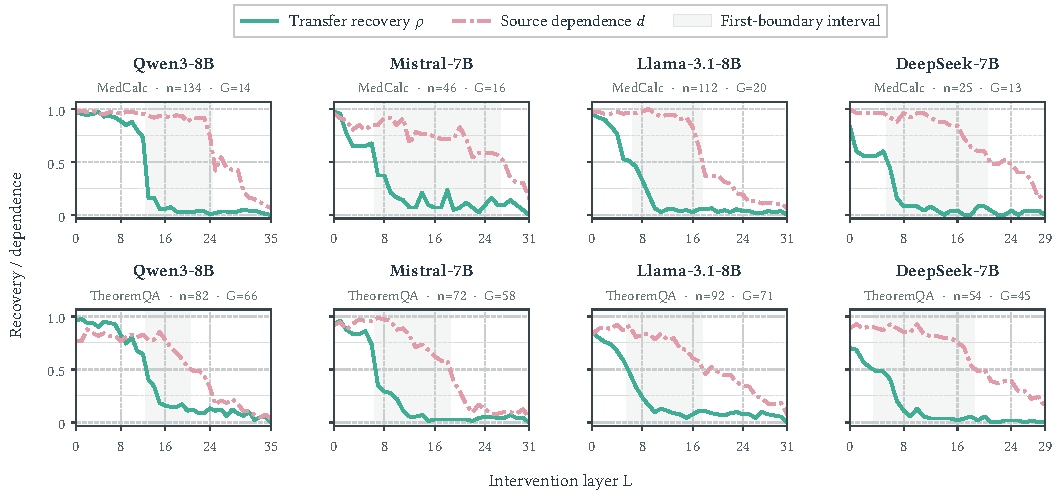
\includegraphics[width=\textwidth]{fig-transfer-reading.pdf}
\caption{State transfer weakens before source-attention dependence across
eight combinations of model and task. Rows show MedCalc (top) and TheoremQA
(bottom), with models aligned by column. Mint: recovery $\rho(L)$ in the wrong-skill
receiver. Pink dash-dotted: dependence $d(L)$ in the original correct-skill
run. Each panel uses common eligible questions with each protocol's own
baselines. $G$ counts skills. Shading spans the first half-effect boundaries
(Table~\ref{tab:paireddepth}). Later threshold crossings remain visible. Knockout
blocks both skill reading and within-skill attention. Every layer is measured.}
\Description{Eight compact line plots in two rows and four columns show mint transfer-recovery curves and pink dash-dotted source-dependence curves on common eligible populations. The top row is MedCalc and the bottom row TheoremQA. Columns are Qwen3-8B, Mistral-7B, Llama-3.1-8B and DeepSeek-7B. Light bands mark intervals between first half-effect boundaries.}
\label{fig:transferreading}
\end{figure*}

\begin{table*}[t]
\centering
\caption{Main depth comparison across four open-weight models and two benchmarks.
$n/G$ gives common eligible questions/skill groups. $T$ and $R$ are the first
half-effect crossings for transfer ($\rho<0.5$) and aggregate source dependence
($d\le0.5$). $\Delta=R-T$ is in layers. $\Delta/D$ normalizes the gap
by the model's layer count. All eight cells use audited common-item populations.}
\label{tab:paireddepth}
\normalfont\rmfamily\fontsize{9}{11}\selectfont
\renewcommand{\arraystretch}{1.18}
\setlength{\tabcolsep}{3pt}
\begin{tabular*}{\textwidth}{@{\extracolsep{\fill}}lrrrrrrrrrr@{}}
\toprule
Model & \multicolumn{5}{c}{MedCalc-Bench} & \multicolumn{5}{c}{TheoremQA} \\
\cmidrule(lr){2-6}\cmidrule(l){7-11}
 & $n/G$ & $T$ & $R$ & $\Delta$ & $\Delta/D$ (\%) & $n/G$ & $T$ & $R$ & $\Delta$ & $\Delta/D$ (\%) \\
\midrule
Qwen3-8B & $134/14$ & $13$ & $25$ & $12$ & $33.3$ & $82/66$ & $13$ & $21$ & $8$ & $22.2$ \\
Mistral-7B & $46/16$ & $7$ & $27$ & $20$ & $62.5$ & $72/58$ & $7$ & $19$ & $12$ & $37.5$ \\
Llama-3.1-8B & $112/20$ & $7$ & $18$ & $11$ & $34.4$ & $92/71$ & $6$ & $18$ & $12$ & $37.5$ \\
DeepSeek-7B & $25/13$ & $6$ & $21$ & $15$ & $50.0$ & $54/45$ & $4$ & $19$ & $15$ & $50.0$ \\
\bottomrule
\end{tabular*}

\end{table*}

\paragraph{Content and position controls.}
The paired content controls replace a common prefix length with either
correct-skill or other-skill information. Correct content recovers $0.65$
of the donor's gain, versus $0.05$ for other-skill content. Shuffling source
positions and injecting random vectors of matching length also give little
recovery. The latter is the norm-matched noise control, which preserves
the Euclidean length of the skill-state change. Rescaling
the correct patch to the receiver's norm still recovers $0.87$.
Together, these controls support a role for skill-specific content and
its arrangement.
The expanded table reports the same controls for every model and task.
Since layer $8$ follows the transfer boundary in several cells, its lower
recovery is consistent with Figure~\ref{fig:transferreading}.
An additional layer-$2$ check gives $56.0\%$ to $93.4\%$ span accuracy
across the eight cells, above noise and shuffled-position controls
in each case (Appendix~\ref{app:limits}).

\paragraph{Cross-question transfer.}
\label{sec:whose}
In the main prompt order, the skill precedes the question. Causal attention
prevents those skill states from encoding a later question. We additionally
place the skill after the question and take donor states from other
questions using the same skill. On $151$ eligible items from $17$
calculators, these states recover $0.98$ at layer $8$, close to $1.02$ for
a donor answering the current question. At layer $16$, the values separate
to $0.29$ and $0.49$. Early transfer thus carries information shared across
questions, with greater question sensitivity later. Further content,
controls varying the strength and retained directions of a state change
appear in Appendix~\ref{app:fullscale}.

% Queue the repair display for the page following the depth comparison.
\begin{figure*}[t]
\centering
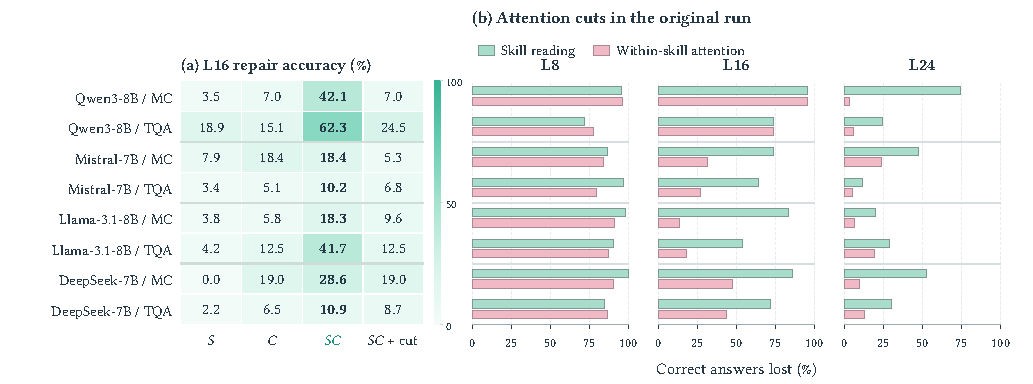
\includegraphics[width=\textwidth]{fig-mechanism-results.pdf}
\caption{Repair and attention cuts across four models and two benchmarks.
MC denotes MedCalc and TQA denotes TheoremQA.
(a) Receiver accuracy at $L16$ for state replacement ($S$), cache
replacement ($C$), joint repair ($SC$), and joint repair with a reading
cut from $L17$ onward ($SC+\mathrm{cut}$).
(b) Correct answers lost in the original correct-skill run under cuts
from $L8$, $L16$ or $L24$ onward during prefill and decoding.
Skill reading blocks reader-to-source attention. Within-skill attention
blocks source-to-source attention. Each row uses the same
questions in both panels, with counts in Table~\ref{tab:mechanism-contrasts}.
Layer numbers index each model's blocks.}
\Description{Eight shared rows pair each of four models with MedCalc and TheoremQA. The left mint heatmap gives all 32 repair accuracies at layer 16 on a fixed zero-to-100-percent scale, with the joint-repair column bold. Three aligned panels on the right show 48 horizontal bars at layers 8, 16 and 24. Mint bars denote Skill reading cuts and pink bars denote Within-skill attention cuts. All three horizontal axes run from zero to 100 percent of originally correct answers lost. At layer 24, reading cuts cause larger losses than within-skill cuts in all eight rows, with varying magnitudes.}
\label{fig:mechanism}
\end{figure*}

\begin{samepage}
\subsection{Weak transfer with persistent source dependence}
\label{sec:where}
\label{sec:depth}
\label{sec:ladder}

\paragraph{Depth separation.}
Early transfer is effective, but it weakens before source dependence does.
Figure~\ref{fig:transferreading} shows the full curves, and
Table~\ref{tab:paireddepth} summarizes their boundaries.
\end{samepage}

The dependence boundary follows the transfer boundary in all eight
comparisons. The gaps are $8$ to $20$ layers, or $22.2\%$ to $62.5\%$ of
model depth (Table~\ref{tab:paireddepth}). The common direction spans
both benchmarks and all four model families.

\paragraph{A representative depth profile.}
For Qwen3-8B/MedCalc, recovery drops from $0.73$
at layer $12$ to $0.16$ at $13$ and stays below $0.08$ from $15$ onward.
Dependence remains $0.93$ at $13$ and $0.75$ at $24$.
Throughout layers $13$ to $24$, transfer restores less than half of the
donor's gain while knockout removes more than half of the originally
correct answers (Figure~\ref{fig:transferreading}).

\paragraph{Paired outcomes and robustness.}
The separation also occurs within questions. In the Qwen3-8B/MedCalc
paired check, $100/124$
($80.6\%$) fail both interventions at layer $13$, and $113/124$ ($91.1\%$)
at $16$ (Appendix~\ref{app:joint-failure}). The boundary ordering also
holds at thresholds $0.4$ and $0.6$ in all eight comparisons. Broader
screening and later threshold crossings appear in Appendix~\ref{app:fullscale}.

\subsection{Partial restoration with source-cache replacement}
\label{sec:mechanism}

\paragraph{Testing an omitted source component.}
Figure~\ref{fig:mechanism} compares all eight model and task combinations,
separating receiver repair at $L16$ (panel a) from attention cuts in the
original correct-skill run at $L8$, $L16$ and $L24$ (panel b).

\paragraph{Repair gains in the receiver.}
Adding caches improves accuracy over state transfer alone in all eight
layer-$16$ comparisons, by $6.8$ to $43.4$ percentage points
(Figure~\ref{fig:mechanism}a). Joint-repair accuracy ranges from $10.2\%$
to $62.3\%$. For Qwen3-8B/MedCalc, $S$, $C$ and $SC$ answer $4$, $8$
and $48$ of $114$ questions correctly ($3.5\%$, $7.0\%$, $42.1\%$).
The cache benefit is $\Delta_{\mathrm{cache}}=(48-4)/114$, or $38.6$
percentage points. The accuracy interaction is
$\Gamma=(48-4-8+0)/114$, or $31.6$ points (Eq.~\eqref{eq:repair-effects}).
At layer $24$, $SC$ reaches $25.4\%$, versus $0.9\%$ for $S$ and
$18.4\%$ for $C$. The added benefit of states alongside caches varies.
For Mistral/MedCalc at $L16$, $SC$ and $C$ both reach $18.4\%$, with
$\Gamma=-7.9$ points. Table~\ref{tab:mechanism-contrasts} reports all
individual conditions and contrasts.

\paragraph{Reading under joint repair.}
Reading cuts reduce joint-repair accuracy by $2.2$ to $37.7$ points
across all eight layer-$16$ comparisons. For Qwen3-8B/MedCalc, accuracy falls
from $42.1\%$ to $7.0\%$, giving $\Delta_{\mathrm{read}}=(48-8)/114$,
or $35.1$ points. Thus the cross-model improvement from adding caches
coexists with continued use of the skill. The Qwen3-8B/MedCalc result at
$L24$ differs: the cut gives $27.2\%$ versus $25.4\%$ without it.
Appendix~\ref{app:mechanism} documents the layer grid and checks sensitivity
to outputs stopped at the generation limit.

\paragraph{Attention paths in the original run.}
Figure~\ref{fig:mechanism}(b) tests the original correct-skill execution.
At $L8$, both types of cut cause large losses across the eight rows.
At $L24$, Skill reading loses $11.9\%$ to $74.6\%$ of correct answers,
exceeding Within-skill attention by $6.8$ to $71.1$ points in every row.
The Qwen3-8B/MedCalc contrast is $74.6\%$ versus $3.5\%$.
At this measured depth, later positions' access to the skill has a
larger effect than attention among skill positions across all eight settings.

% Let the discussion follow the results without forcing a new column.
\section{Discussion}
\label{sec:discussion}

\paragraph{Potential applications.}
Our findings suggest a way to evaluate the reuse of contextual skills.
Consider a Web agent that repeatedly follows the same instructions across
requests. A reusable internal representation would need to preserve task
performance in the receiving execution. Our results motivate evaluating
this transfer separately from the original execution's dependence on the
skill. If a reuse method also removes access to the original instructions,
that additional change needs its own evaluation. The observed cache gains
motivate reuse methods that carry both hidden states and attention caches
across requests. Deployment studies can evaluate their latency, memory
use and task performance in interactive Web settings.

\paragraph{Future work.}
A next step is to investigate which questions benefit from cache
replacement. The mathematical analysis connects remaining cache
differences to output stability under explicit assumptions. Measuring
these differences, their influence on token predictions and the donor's
prediction margins could test whether this framework helps distinguish
successful from unsuccessful repairs. Another direction is to separate
the effects of cache content and layer coverage through matched other-skill
copies and additional layer ranges. Separating attention cuts during prompt
processing from those during answer generation would clarify when continued
skill access matters. Finally,
testing neutral receiving contexts and multi-step Web workflows would
assess how far the observed separation extends beyond the screened
question-answering settings studied here.

\section{Conclusion}
\label{sec:conclusion}

Using a contextual skill and reusing its internal states are distinct
capabilities. Across four models and two benchmarks, state transfer
weakens before the original execution's dependence on skill attention,
with half-effect boundaries separated by $8$ to $20$ layers.
Early content controls establish that the transferred states carry
skill-relevant information, and the depth comparisons show that this
information becomes harder to reuse while the skill remains useful.

Source-cache replacement provides a way to recover part of that transfer.
At layer $16$, adding caches improves accuracy over states alone by
$6.8$ to $43.4$ percentage points in all eight comparisons, while cutting
subsequent skill reading reduces the joint-repair accuracy in each.
The mathematical analysis connects cache alignment to output stability
under explicit conditions. Together, these findings motivate evaluating
state reuse separately from continued skill use and including cached
information in the design of reusable skill representations.

\label{endmain}

\bibliographystyle{ACM-Reference-Format}
\bibliography{skillvector}

%% ================================================================= appendix
\appendix
%% Compact appendix: what a reader needs to reproduce or scope the result.
\begin{table*}[tbp]
\caption{Screening and full-pool rerun for Qwen3-8B/MedCalc at layer $8$.
Entries show recovery
(Eq.~\ref{eq:rho}). The group screen keeps calculators whose receiver
solves no sampled question. The item screen keeps individual receiver
failures. Category means related calculator functions. Direction and
quarter controls are defined in Appendix~\ref{app:fullscale}.
Each condition uses its own matched baselines. ``Not run'' marks an
unmeasured condition.}
\label{tab:fullscale}
\centering
\small
\renewcommand{\arraystretch}{1.18}
\begin{tabular}{lccc}
\toprule
Intervention & Full, group screen ($n=135$) & Subset ($n=60$) & Full, item screen ($n=369$) \\
\midrule
Correct skill span & $\mathbf{0.89}$ & $0.87$ & $0.94$ \\
same skill, matched prefix & $0.65$ & $0.73$ & $0.84$ \\
\midrule
Half-strength change $\alpha=0.5$ & $0.04$ & $0.06$ & $0.11$ \\
positions permuted & $0.05$ & $0.08$ & $0.21$ \\
norm-matched noise & $0.02$ & $0.10$ & $0.18$ \\
other calculator & $0.05$ & Not run & $0.25$ \\
other calculator category, mean & $0.05$ & $0.06$ & $0.16$ \\
same calculator category, mean & $0.12$ & $0.05$ & $0.24$ \\
identity patch & $0.00$ & $0.00$ & $0.00$ \\
\midrule
Leading directions: $128/64/32/16$ & $0.77/0.63/0.12/0.05$ & $0.77/0.54/0.13/0.06$ & $0.88/0.70/0.22/0.18$ \\
Least prominent directions: $64/16$ & $0.03/0.04$ & $0.00/0.06$ & $0.11/0.12$ \\
Skill quarters: $1/2/3/4$ & $0.09/\mathbf{0.56}/0.12/0.05$ & $0.12/0.56/0.12/0.12$ & $0.18/0.64/0.22/0.19$ \\
\bottomrule
\end{tabular}
\end{table*}

% Appendix A: protocol, implementation and scope.
\section{Experimental protocols and provenance}
\label{app:setup}

\paragraph{Tasks and scoring.}
MedCalc provides $55$ calculator skills and $20$ questions per calculator
through SRA-Bench, scored against prescribed numerical tolerances.
TheoremQA uses its released prompts, skill assignments and evaluator.
Skills are supplied directly, with no tools during generation.
Groups are calculators for MedCalc and skill identities for TheoremQA.

\paragraph{Evaluation populations.}
The original MedCalc list contains $470$ previously rescued questions,
answered incorrectly without a skill and correctly with one. Eligibility
restrictions leave $467$ from $48$ calculators for corrected transfer controls.

The group screen retains skills with no correct receiver answers,
including donor failures. Its $135$ questions from $14$ calculators yield
$124$ correct donor and $110$ correct layer-$8$ span answers.
Recovery uses the measured donor gain. Intersection with knockout's
correct-with-skill, incorrect-without-skill IDs gives $134$ depth items,
with separate intervention baselines.

The seven added control cells require a fresh correct donor and incorrect
no-skill baseline, giving $100\%$ donor accuracy. Repair instead screens
individual items. Of $124$ candidate IDs, $116$ are donor-correct and
receiver-incorrect, and $114$ also fail without the skill. Repair and path
cuts share these $114$. The candidate, paired-check and correct-donor
counts each equal $124$ under different, non-interchangeable rules.

The broader screen in Appendix~\ref{app:fullscale} retains individual
receiver failures. Other-skill and noise interventions are more effective
under this broader screen, as reported in
Table~\ref{tab:fullscale}. The common DeepSeek/MedCalc depth set contains
$25$ questions, so its boundary may be sensitive to sample composition.
Changing the half-effect threshold tests the summary rule, not that
sampling sensitivity.

\subsection{Implementation details}
\label{app:detail}

\paragraph{Wrong-skill selection and token matching.}
Each dataset uses one fixed distractor. MedCalc uses APACHE II, a clinical
severity score (\texttt{medcalcbench\_043}), as a long distractor outside the
selected calculators. TheoremQA uses
\texttt{theoremqa\_148}, a mathematical skill about representation theorems
and differential equations, selected by fewest assigned questions, then
greatest document length. Its assigned items are excluded.
We repeat the distractor's tokens if needed and copy the first $m$ into
the target span of width $m$, without padding. All other tokens and
positions remain unchanged. This context may repeat or truncate the
alternative skill.

\paragraph{Prompt and source boundaries.}
The user turn has the order \texttt{Relevant Skill:}, skill text, a blank
line, and the benchmark's question prompt. MedCalc appends the instruction
to show calculations and end with \texttt{ANSWER: <your answer>}.
Its system message asks for a step-by-step score calculation from a patient
note. TheoremQA retains the benchmark's science-teacher system message,
\texttt{Problem:<question>} and \texttt{Solution:} user format, and
``Therefore, the answer is ...'' final-answer requirement.
The tokenizer converts text to tokens. Its chat template supplies role
labels and the generation prompt. Character offsets identify tokens
overlapping the skill text, excluding its header and separator.
We replace IDs in $[\mathrm{lo},\mathrm{hi})$, including the start but
excluding the end, without decoding and retokenizing.

\paragraph{Models and decoding.}
The four main models are Qwen3-8B ($36$ layers, hidden width $4096$),
Mistral-7B-Instruct-v0.3 ($32$ layers, width $4096$),
Llama-3.1-8B-Instruct ($32$ layers) and DeepSeek-LLM-7B-Chat ($30$ layers).
Llama and DeepSeek state capture and knockout use BF16, a 16-bit
floating-point format, and $900$ new tokens. Both use eager attention,
which explicitly computes attention scores and applies the mask,
without further reducing weight precision. DeepSeek and Mistral merge
system instructions into the user turn. Llama uses the original weights,
configuration and vocabulary with the public distribution's tokenizer
template. Decoding is greedy, with Qwen's extended-reasoning mode disabled.
Earlier state replacement uses PyTorch scaled dot-product attention (SDPA).
Regenerated Qwen and Mistral TheoremQA runs use SDPA for transfer, eager
attention for knockout and $900$ new tokens. Historical Qwen3-8B/MedCalc also
allows $900$ tokens in both runs, with different attention implementations.
Repair and path experiments use BF16, eager attention and $1{,}536$ new
tokens. All their conditions split prefill before the final prompt token,
allowing cache writes before its recomputation.
All cuts span prefill and decoding. Layer indices in the path comparisons
refer to the measured blocks, not matched computational stages across models.

\paragraph{Position and state checks.}
Length matching preserves question positions. Patches replace prefill
block outputs indexed separately from scored answer tokens. Identity
controls write back receiver states. A final-layer patch reproduces donor
next-token scores at that position. Cuts preserve the causal mask.

\paragraph{Checking the prefill procedure.}
A preliminary comparison of full and split prefill uses one item from each
of $14$ calculators. All $84$ own-state checks reproduce receiver tokens
exactly. Changing prefill changes one donor's and one receiver's
correctness, motivating fresh baselines under the common split protocol.
Result records retain truncation counts and sensitivity analyses.

\subsection{Evaluation scope and intervention provenance}
\label{app:limits}

\paragraph{Attention-mask correction.}
State capture originally omitted the decoding attention mask. These
mathematically equivalent calls for unpadded sequences selected different
numerical implementations, producing state differences of $1.2\%$ at layer
$8$ and $25\%$ at $34$. Identity patching changed $108/1{,}766$ Qwen3-8B
outcomes ($6.1\%$). Matching masks restores exact identity agreement,
including all $467$ corrected MedCalc items. All main state interventions
use this correction. Knockout modifies masks without donor-state capture.

\paragraph{Development and replication.}
Initial MedCalc controls sampled four rescued questions from each of the
$40$ largest eligible calculator groups. The corrected Qwen3-8B rerun
uses all rescued questions from groups with at least two
(Table~\ref{tab:fullscale}). The eight-cell depth study uses common items
for both interventions.

\paragraph{Extension pools and grading checks.}
The Llama and DeepSeek extensions use frozen pools of $446$ MedCalc and
$255$ TheoremQA questions inherited from earlier models' eligible transfer
items. Each model is screened again on its own unpatched baselines.
One DeepSeek/MedCalc candidate cannot reserve $900$ answer tokens and is
excluded before inference. TheoremQA regrading uses official rules,
resetting the parser per answer. Reversed-order and separate-process checks
agree before eligibility is recomputed.
Qwen3-8B and Mistral TheoremQA regeneration uses $168$ and $142$ frozen
candidates, yielding $82/66$ and $72/58$ common questions/skills.
Neither audit finds grading changes, missing common layer entries or
identity failures. Reverse-order and $16$ separate-process checks per model agree.

Layer-$2$ controls use their own screened sets. In the model order of
Table~\ref{tab:probe}, the MedCalc question counts are $97,35,112,25$ and
correct-span counts are $87,24,101,14$. TheoremQA counts are $61,61,92,54$,
with $57,52,70,31$ correct. The DeepSeek/TheoremQA cells use the final
$54$-item grading correction.

\paragraph{Artifact availability.}
Stored artifacts contain configurations, question IDs, answers and token
sequences. An anonymous review archive is not yet linked.




% Full-data rerun; its wide table is queued at the appendix entrance.
\section{Additional transfer and source-dependence analyses}
\label{app:fullscale}

\begin{table*}[t]
\centering
\caption{Source-cache repair at layer $16$ across four models and two benchmarks.
$n/G$ counts questions and skills retained using fresh baselines.
$S$, $C$, $SC$ and $SC+\mathrm{cut}$ show accuracy (\%).
The last three columns show cache benefit $\Delta_{\mathrm{cache}}$,
accuracy interaction $\Gamma$ and reading-cut loss $\Delta_{\mathrm{read}}$
in percentage points (Eq.~\eqref{eq:repair-effects}). Each row uses the
same questions for all conditions, with donor accuracy $100\%$ and
receiver accuracy $0\%$. These populations differ from Table~\ref{tab:paireddepth}.}
\label{tab:mechanism-contrasts}
\normalfont\rmfamily\fontsize{9}{11}\selectfont
\renewcommand{\arraystretch}{1.18}
\setlength{\tabcolsep}{2.5pt}
\begin{tabularx}{\textwidth}{@{}ll*{8}{>{\centering\arraybackslash}X}@{}}
\toprule
\rowcolor[HTML]{E4F4FA}
Model & Task & $n/G$ & $S$ & $C$ & $SC$ & $SC+\mathrm{cut}$ & $\Delta_{\mathrm{cache}}$ & $\Gamma$ & $\Delta_{\mathrm{read}}$ \\
\midrule
Qwen3-8B & MedCalc & $114/14$ & 3.5 & 7.0 & \textbf{42.1} & 7.0 & $+38.6$ & $+31.6$ & $+35.1$ \\
Qwen3-8B & TheoremQA & $53/43$ & 18.9 & 15.1 & \textbf{62.3} & 24.5 & $+43.4$ & $+28.3$ & $+37.7$ \\
\addlinespace[2pt]
Mistral-7B & MedCalc & $38/15$ & 7.9 & 18.4 & \textbf{18.4} & 5.3 & $+10.5$ & $-7.9$ & $+13.2$ \\
Mistral-7B & TheoremQA & $59/49$ & 3.4 & 5.1 & \textbf{10.2} & 6.8 & $+6.8$ & $+1.7$ & $+3.4$ \\
\addlinespace[2pt]
Llama-3.1-8B & MedCalc & $104/20$ & 3.8 & 5.8 & \textbf{18.3} & 9.6 & $+14.4$ & $+8.7$ & $+8.7$ \\
Llama-3.1-8B & TheoremQA & $72/56$ & 4.2 & 12.5 & \textbf{41.7} & 12.5 & $+37.5$ & $+25.0$ & $+29.2$ \\
\addlinespace[2pt]
DeepSeek-7B & MedCalc & $21/10$ & 0.0 & 19.0 & \textbf{28.6} & 19.0 & $+28.6$ & $+9.5$ & $+9.5$ \\
DeepSeek-7B & TheoremQA & $46/40$ & 2.2 & 6.5 & \textbf{10.9} & 8.7 & $+8.7$ & $+2.2$ & $+2.2$ \\
\bottomrule
\end{tabularx}
\end{table*}


The original Qwen3-8B/MedCalc controls sampled four rescued questions
from each of $40$ calculators ($160$ items). The group screen retained
$60$ from $15$ calculators. The rerun used all $467$ eligible questions
from $48$ calculators with the same interventions. Screening whole
groups now requires failure on up to $20$ questions instead of four,
retaining $135$ from $14$ calculators. Screening each item separately
retains $369$ from $45$ calculators (Table~\ref{tab:fullscale}).

For the dose and rank controls in Table~\ref{tab:fullscale}, the state
difference is $\delta^L=H_D^L[\mathcal I]-H_R^L[\mathcal I]$.
The rank implementation preserves the mean over source positions.
Let $\bar\delta^L$ repeat that mean at every row, and define
$\delta_k^L=\bar\delta^L+(\delta^L-\bar\delta^L)_k$, where
$(\cdot)_k$ retains the leading $k$ components of a singular value
decomposition, which ranks directions by how much matrix variation they capture.
The dose and rank controls share the notation
\begin{equation}
H_R^L[\mathcal I]\leftarrow H_R^L[\mathcal I]+\alpha\delta_k^L.
\label{eq:dose-rank}
\end{equation}
Full rank with $\alpha=1$ is full replacement, and $\alpha=0.5$ is half
the state difference. Rank controls use $\alpha=1$.
Increasing $k$ from $32$ to $64$ restores much of the recovery.
A bottom-$k$ control instead retains the least prominent directions of
the centered variation, with the same mean retained.
The second of four equal portions of the skill, containing its formula,
gives the largest recovery when copied alone in both samples.
The same-category mean donor changes from $0.05$ to $0.12$, on the $41$
full-rerun items where it is available. Here category refers to a calculator
group derived from skill-title keywords (for example, related fluid calculations). The intervention averages
donor-minus-receiver state differences from other calculators in that group.

\paragraph{The depth sweep at one-layer resolution.} The subset sweep measured
layers $0,4,8,12,14,15,16,20$ and placed the collapse somewhere after $12$.
At full scale we added $13$ and $17$ to $19$:
recovery is $0.98,0.98,0.89,0.74$ at layers $0,4,8,12$, then
$0.16,0.16,0.06,0.06,0.07,0.03,0.02,0.03$ at $13$ through $20$ under the group screen.
The item screen gives $1.00,0.98,0.94,0.79$ then
$0.32,0.34,0.25,0.25,0.23,0.19,0.14,0.17$.
Both screens show their largest local decline
between layers $12$ and $13$.

\paragraph{Broader screening and boundary sensitivity.}
The item-level screen retains the transfer decline. Paired knockout
comparisons use the common-item populations. Using transfer thresholds
$\tau=0.4$ or $0.6$ with dependence thresholds $1-\tau$ preserves the
boundary ordering in all eight main comparisons. Qwen3-8B/MedCalc dependence
first falls to at most half at layer $25$, rises above half again at $26$,
and remains below half from $27$ onward. The curves retain these recrossings.

\paragraph{Same-question joint failures.}
\label{app:joint-failure}
This check requires correct donors under both protocols, an incorrect
transfer receiver and an incorrect no-skill knockout baseline.
Joint failures at the transfer boundary are $100/124$ ($80.6\%$) for
Qwen3-8B at $T=13$ and $25/43$ ($58.1\%$) for Mistral-7B at $T=7$,
on $14$ and $15$ MedCalc skill groups. These sets differ from
Table~\ref{tab:paireddepth}. Four items in each pass the transfer
no-skill baseline despite failing it under knockout.

\paragraph{Repeated replacement as a consistency check.}
\label{app:repeated}
On the $135$ screened MedCalc items, replacing source states at layers
$8$ to $11$, $12$ to $15$, $14$ to $19$ and $16$ to $35$ recovers
$0.89,0.74,0.16,0.06$. Starting at the first layer recovers $0.98$.
Repeated and single writes produce identical tokens from each starting
layer, consistent with Appendix~\ref{app:cache-coverage}'s causal argument.

\paragraph{A continuous readout at the same boundary.}
We generate correct-skill reasoning once per item, then score that fixed
sequence under each intervention. This is teacher forcing: recorded
preceding tokens replace newly generated ones. Mean token log-probability
uses natural logarithms, measured in nats. Higher values indicate stronger
predictions of the recorded sequence. We normalize it as
$z=(\ell_L-\ell_{\mathrm{recv}})/(\ell_{\mathrm{gold}}-\ell_{\mathrm{recv}})$,
where $\ell$ is the mean log-probability for the patched, receiver or
donor condition. This $z$ differs from knockout retention $q$.

On $442$ donor-correct items from $48$ calculators, $z$ is
$0.999,0.989,0.960,0.831,0.598,0.595,0.340,0.201,0.129$ at layers
$0,4,8,12,13,14,16,20,24$. The $0.233$ drop from $12$ to $13$ is near
the accuracy boundary in the separate $134$-item depth set.
The decline spans all four quarters of the reasoning sequence
($0.20,0.26,0.31,0.21$). After supplying the reasoning, all conditions
predict the final number closely: median log-probabilities lie between
$-0.001$ and $-0.005$. Their donor-minus-receiver denominator has median
$0.0014$ and is below $0.01$ on $59\%$ of items, limiting this readout.

\paragraph{Distributed reading and receiver state.}
The attention output contributed by skill positions,
normalized by the length of the hidden-state vector, concentrates in
layers $12$ to $21$. Blocking the $32$ highest-ranked
heads costs $0.39$ of the skill's effect, versus $0.23$ for random heads at the
same layers (calculators not used to rank the heads, paired difference $0.154$). Reading uses many heads rather than a small subset. After late span replacement, the attention output from skill positions remains
$0.86$ to $0.99$ of the donor's despite weak behavioural recovery. Earlier receiver question-state updates remain unchanged, motivating
the interaction tests in \S\ref{sec:mechanism}.


\subsection{Source-cache repair and attention-path experiments}
\label{app:mechanism}

The focused Qwen3-8B/MedCalc experiments fix $\mathcal Q_0$, comprising
$124$ historical IDs from $14$ calculators, before inference. Four NVIDIA
RTX 4090 graphics processors each receive every fourth ID, using the
$1{,}536$-token protocol in Appendix~\ref{app:detail}.
Let $e_i^X$ be binary correctness for item $i$ in condition $X$, with
$0$ denoting no skill. Selection uses only fresh baselines:
\begin{equation}
\mathcal Q_{\mathrm{rep}}
=\{i\in\mathcal Q_0:e_i^D=1,\ e_i^R=e_i^0=0\}.
\label{eq:repair-set}
\end{equation}
Of $116$ donor-correct, receiver-incorrect items, $114$ also fail without
a skill. On these same $114$ items, every condition uses
$a_X(L)=|\mathcal Q_{\mathrm{rep}}|^{-1}
\sum_{i\in\mathcal Q_{\mathrm{rep}}}e_i^X(L)$.
All $372$ baseline generations agree
token-for-token between the two suites. The complete repair grid contains
$2{,}356$ generations, the path grid $1{,}488$, and worker identity checks
$100$. All $48$ own-state writebacks are token-exact.

Figure~\ref{fig:mechanism} and Table~\ref{tab:mechanism-contrasts} use this
rule for eight comparisons with separate candidates. Repair and path tests
share item IDs and baseline tokens within each row. Repair is measured
at $L8$, $L12$, $L16$ and $L24$, and path cuts at $L8$, $L16$ and $L24$.
Writes, masks and contrasts follow
Eqs.~\eqref{eq:cache}, \eqref{eq:reading-cut} and \eqref{eq:repair-effects}.

\paragraph{Qwen3-8B/MedCalc truncation sensitivity.}
We retain all intervention outcomes, including outputs stopped at the
generation limit, which we call truncated outputs. For the
prespecified difference between $SC$ and $S$ at layer $16$, the gain is $38.6$ percentage
points.
The corresponding accuracy interaction $\Gamma$ is $31.6$ points. $SC-(SC+\mathrm{cut})$ is $35.1$ points.
On the $96$ items with all three baselines untruncated, the $SC$ gain over $S$ is
$38.5$ points.
At layer $16$, $S$, $SC$ and $SC+\mathrm{cut}$ truncate $4$, $4$ and $3$ of $114$ outputs.
Scoring truncated $S$ answers as correct and truncated $SC$ answers as
incorrect still leaves a
$35.1$-point repair advantage. At layer $24$, $SC$ and $SC+\mathrm{cut}$ truncate $3$ and $28$
outputs and show no additional loss in measured accuracy.

At layer $24$, reader and source-self cuts retain $29/114$ and $110/114$
correct answers. Their loss difference is $71.1$ points.
Reader cuts truncate $21$ outputs. Counting all as correct still leaves
retention at $50/114$, below source-self retention $110/114$ (no truncation).
Both contrasts survive this worst-case reassignment. Experiment records retain counts for each condition, file checksums
and these sensitivity calculations.

\paragraph{Redundant combined cut.}
With causal attention and otherwise positionwise operations, earlier
tokens cannot read the skill. Persistent reading cuts also prevent its
changed states from reaching later tokens. Adding a within-skill cut
therefore leaves outputs unchanged by induction over layers and generated
tokens. We omit this redundant condition. The argument does not apply
when later reading is allowed.

\subsection{Cache coverage under causal prefill}
\label{app:cache-coverage}

This deduction assumes a deterministic causal Transformer with masked
attention as its only cross-position operation
\citep{vaswani2017attention}, identical parameters and position IDs,
and the same exact-arithmetic computation without extra attention cuts.
Donor and receiver tokens differ only within the complete, contiguous
source interval $\mathcal I=[\mathrm{lo},\mathrm{hi})$ in the prefix.

\paragraph{Proposition (source-cache coverage).}
Suppose $S$ replaces the entire source output of block $L$ before the
next block executes, and the cache write occurs only after prefix prefill.
At the observation point in Eq.~\eqref{eq:continuation},
\begin{equation}
\mathcal C_S^\ell[\mathcal I]=
\begin{cases}
\mathcal C_R^\ell[\mathcal I],&\ell\le L,\\
\mathcal C_D^\ell[\mathcal I],&\ell>L.
\end{cases}
\label{eq:source-coverage}
\end{equation}
Together with the explicit write at layers $0$ through $L$, this gives
$\mathcal C_{SC}[\mathcal I]=\mathcal C_D[\mathcal I]$.

\emph{Proof.}
Block-$L$ KV is computed before the output patch, leaving source caches
at $\ell\le L$ unchanged. Before $\mathrm{lo}$, identical tokens and
causality give identical states at every layer. After $S$, all block-$L$
outputs at $i<\mathrm{hi}$ therefore match the donor.
At these positions, the next block reads only matching earlier or
current states, producing matching source KV and outputs.
Induction proves the upper-layer case.
Equation~\eqref{eq:cache} supplies the lower layers for $SC$.
\hfill$\square$

\begin{table}[t]
\centering
\caption{Prefix-cache coverage before the final prompt token, assuming
deterministic causal computation in exact arithmetic and a complete,
contiguous source span with aligned positions and identical preceding
tokens. $D$ and $R$
denote donor and receiver source KV. $\mathcal B_R$ and $\mathcal B_S$
are all other prefix caches from the unpatched and state-patched runs.
The entries are identities derived under these assumptions.}
\label{tab:cache-coverage}
\small
\renewcommand{\arraystretch}{1.18}
\setlength{\tabcolsep}{5pt}
\begin{tabular}{@{}lccc@{}}
\toprule
Condition & \multicolumn{2}{c}{Source KV} & Other KV \\
\cmidrule(lr){2-3}
 & $\ell\le L$ & $\ell>L$ & All layers \\
\midrule
Receiver & $R$ & $R$ & $\mathcal B_R$ \\
$S$ & $R$ & $D$ & $\mathcal B_S$ \\
$C$ & $D$ & $R$ & $\mathcal B_R$ \\
$SC$ & $D$ & $D$ & $\mathcal B_S$ \\
\bottomrule
\end{tabular}
\end{table}


\paragraph{Remaining execution state.}
The post-prefill write preserves the other caches
(Table~\ref{tab:cache-coverage}). Under these assumptions,
\begin{equation}
\begin{aligned}
\hat y_{SC}&=\mathcal G_{\theta,M_0}
 (u_*,\mathcal C_D[\mathcal I],\mathcal B_S),\\
\hat y_D&=\mathcal G_{\theta,M_0}
 (u_*,\mathcal C_D[\mathcal I],\mathcal B_D),
\end{aligned}
\label{eq:source-not-full}
\end{equation}
where $M_0$ is the original mask. Since $\mathcal B_S$ need not equal
$\mathcal B_D$, answers may differ. All-layer source-KV-only replacement
instead preserves $\mathcal B_R$ and is generally not equivalent to $SC$.

Under $SC+\mathrm{cut}$, source queries remain unmasked, so the same
induction applies. However, $\mathcal B_{SC+\mathrm{cut}}$ may differ
from $\mathcal B_S$, and continuation uses a different mask. The contrast
includes both prefill and decoding effects.

Code inspection confirms the stated write ordering. Exact source-cache
identities rely on the arithmetic assumption above. Discrepancies against
the donor in BF16 runs remain unmeasured.

\subsection{A sufficient condition for behavioral recovery}
\label{app:behavior-recovery}

We apply margin-based stability reasoning \citep{tsuzuku2018lipschitz}
to cached decoding, adding a sensitivity assumption to Eq.~\eqref{eq:cache-distance}.

\paragraph{One-step guarantee.}
Fix the model, last prompt token $u_*$, positions and original mask $M_0$.
For vocabulary $\mathcal V$, let $F(\mathbf z)\in\mathbb R^{|\mathcal V|}$
map initial prefix caches to next-token logits. Assume finite sensitivity
$\kappa$ over the compared states in $\Omega$. The infinity norm is the
largest absolute change in any token score:
\begin{equation}
\|F(\mathbf z)-F(\mathbf z')\|_\infty
\le\kappa\|\mathbf z-\mathbf z'\|_2,\qquad
\mathbf z,\mathbf z'\in\Omega.
\label{eq:cache-lipschitz}
\end{equation}
For the donor's unique greedy choice $y_D$, define its positive margin
\begin{equation}
m_D=F_{y_D}(\mathbf z_D)-\max_{v\ne y_D}F_v(\mathbf z_D)>0.
\label{eq:donor-margin}
\end{equation}
\emph{Proposition.} If $2\kappa\varepsilon_{SC}<m_D$, then greedy
decoding from $\mathbf z_{SC}$ selects $y_D$.
\emph{Proof.} Each logit changes by at most
$\kappa\varepsilon_{SC}$. Thus, for every $v\ne y_D$,
\begin{equation}
F_{y_D}(\mathbf z_{SC})-F_v(\mathbf z_{SC})
\ge m_D-2\kappa\varepsilon_{SC}>0.
\label{eq:margin-preservation}
\end{equation}
The factor $2$ allows the winning logit to decrease and a competitor
to increase. Strict inequality excludes ties. \hfill$\square$

\paragraph{Complete generation.}
Let the donor produce $N$ tokens including its stopping token.
$F_t^D(\mathbf z)$ processes $u_*$ and fixed donor history $y_{D,<t}$
from initial cache $\mathbf z$, recomputing all new caches.
Assume Eq.~\eqref{eq:cache-lipschitz} for $F_t^D$ with bound $\kappa_t$
and donor margin $m_{D,t}>0$. The bound includes all intervening cache updates:
\begin{equation}
\bigl[\ \forall t\le N:\ 2\kappa_t\varepsilon_{SC}<m_{D,t}\ \bigr]
\quad\Longrightarrow\quad \hat y_{SC}=\hat y_D.
\label{eq:sequence-recovery}
\end{equation}
The first token agrees by the one-step result. If earlier tokens agree,
decoding follows the history defining $F_t^D$, so token $t$ agrees.
Induction under the common stopping rule gives an identical sequence,
which is correct whenever the donor's answer is correct.

\paragraph{Scope.}
Common valid $\kappa_t$ over $D$, $S$ and $SC$ give $SC$ no larger error
bounds (Eq.~\eqref{eq:cache-distance}). Losing cancellation can increase
actual errors, so accuracy gains are not guaranteed. Different sequences
may answer correctly, making this condition only sufficient.
$SC+\mathrm{cut}$ changes the mask and prefix and is excluded.
Sensitivity bounds and itemwise margins remain unverified.




\end{document}
